\chapter{ArcFace}\label{ch:arcface}
ArcFace~\cite{ArcFace} is a research which became public in 2018 and achieved state-of-the-art results on LFW dataset.
The objective of the research was to design a loss function which solves the main drawbacks of \textit{sofmax loss}
and the \textit{triplet loss}.

There are two issues with \textit{softmax loss}.
The first one is that the dimension of the output weight matrix grows linearly with the number of identities in the
training set.
The second drawback is that the learned features are not discriminative enough for the open-set face recognition
problem.
That means that the model doesn't perform well on not yet seen faces.

The drawbacks of \textit{triplet loss} are the demands entailed by the construction of the triplets.
The number of those is subject to combinatorial explosion.
This is a serious issue especially for large datasets.


\begin{figure}[H]
    \centering
    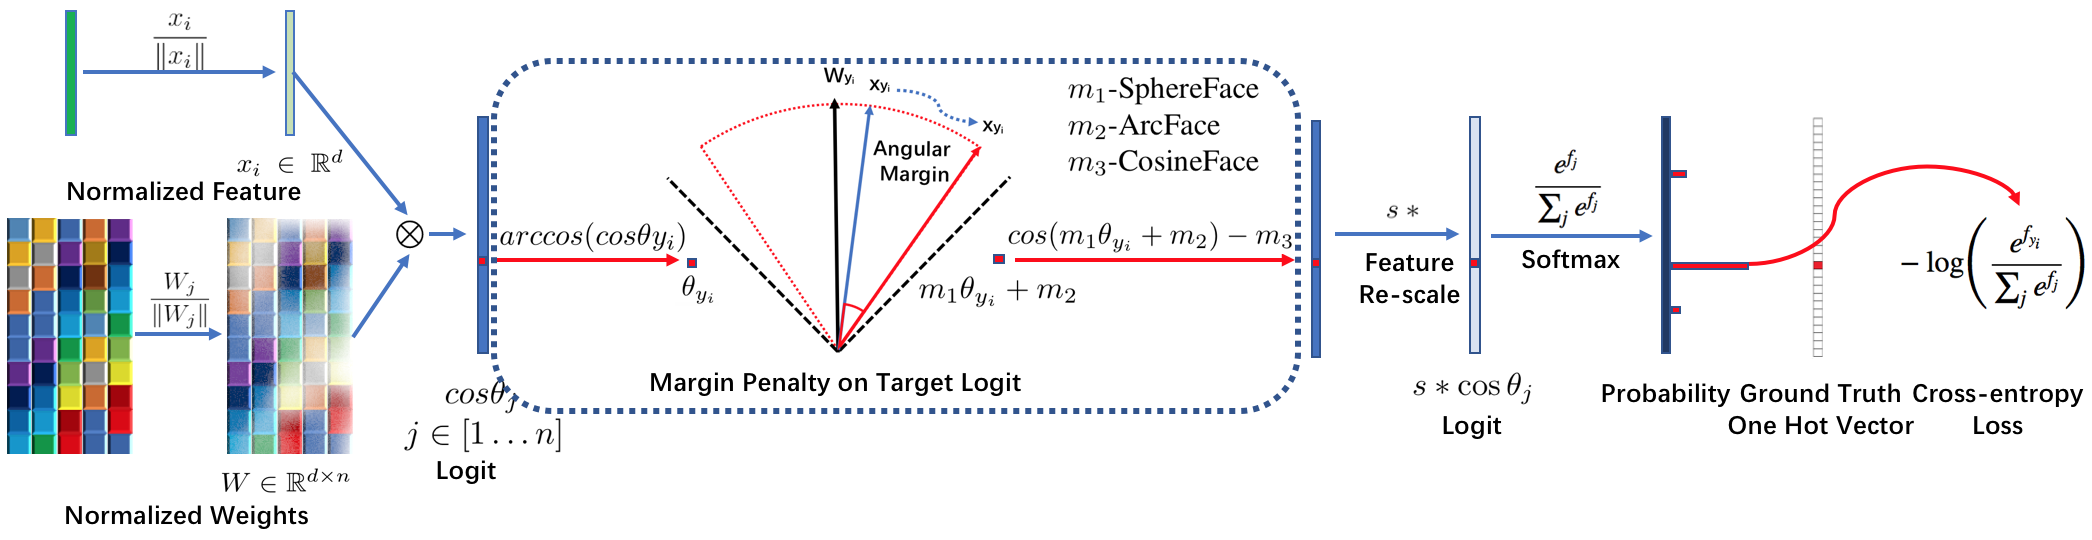
\includegraphics[width=\columnwidth]{images/arcface/arcface.png}
    \caption{Training a CNN for face recognition supervised by the ArcFace loss~\cite{ArcFace}}
    \label{fig:arcface}
\end{figure}